\documentclass[12pt]{article}
    \usepackage[utf8]{inputenc}
    \usepackage{natbib}
    \bibliographystyle{chicago}
    \usepackage{geometry}
    \usepackage{latexsym}
    \usepackage{amsmath,amsthm,amsopn,amstext,amscd,amsfonts,amssymb}
    \usepackage{caption}
    \usepackage{graphicx}
    \usepackage{lscape}
    \usepackage[usenames,dvipsnames]{color}
    \usepackage{epsfig}
    \usepackage{hyperref}
    \usepackage{indentfirst}
    \hypersetup{
        %bookmarks=false,                     % show bookmarks bar?
        unicode=false,  % non-Latin characters in Acrobat’s bookmarks
        pdftoolbar=true,                    % show Acrobat’s toolbar?
        pdfmenubar=true,                  % show Acrobat’s menu?
        pdffitwindow=false,       % window fit to page when opened
        pdfstartview={FitH}, % fits the width of the page to the window
        pdftitle={},                % title
        pdfauthor={F. Vazquez-Grande},      % author
        pdfsubject={},               % subject of the document
        pdfcreator={},               % creator of the document
        pdfproducer={},             % producer of the document
        pdfkeywords={keyword1} {key2} {key3}, % list of keywords
        pdfnewwindow=true,              % links in new window
        colorlinks=true,    % false: boxed links; true: colored links
        linkcolor=NavyBlue,          % color of internal links
        citecolor=NavyBlue,          % color of links to bibliography
        filecolor=magenta,           % color of file links
        urlcolor=NavyBlue            % color of external links
    }
    \usepackage{setspace}
    %\singlespacing
    \onehalfspacing
    \graphicspath{{figs/}}
    % page numbering
    \usepackage{fancyhdr}
    \pagestyle{fancy}
    \renewcommand{\headrulewidth}{0pt}
    \rhead{\thepage}
    \lhead{}
    \cfoot{}
    \usepackage{booktabs}
    \usepackage{algorithm2e}
    \usepackage{appendix}
    \DeclareMathOperator*{\argmin}{arg\,min} % thin space, limits underneath in displays


% Keywords command
\providecommand{\keywords}[1]
{
  \small	
  \textbf{Keywords:} #1
}


\title{Combining forecasts: \\Can machines beat the average?\footnote{The views presented here are solely those of the authors and do not necessarily represent those of Board of Governors of the Federal Reserve or of the Federal Reserve System.}}
\author{Tyler Pike\thanks{Corresponding author. (\texttt{\href{mailto:Tyler.J.Pike@frb.gov}{Tyler.J.Pike@frb.gov}}). 1801 K St NW, Washington, DC 20006} \\ Federal Reserve Board \and Francisco Vazquez-Grande \\ Federal Reserve Board }

\date{\today}

\begin{document}
\maketitle

\begin{abstract}
    %Combining forecasts: A nonlinear path forward \\ 
    Yes. This paper documents the benefits of combining forecasts using weights built with non-linear models.  We introduce our tree-based forecast combinations and compare them with benchmark equal weight combination as well as other nonlinear forecast weights. We find that nonlinear models can improve consistently upon the equal weight alternative--breaking the so-called ``forecast combination puzzle''--and that our proposed methods compete well with other nonlinear methods. \\

    %Conference draft pdf and tex is saved in version folder.
\end{abstract}
\keywords{forecast combination; machine learning; random forest}

\clearpage
%%%%%%%%%%%%%%%%%%%%%%%%%%%%%%%%%%%%%%%

%\section{Outline}

%\textbf{Timmermann Paper outline}
%\begin{enumerate}
%    \item Introduction
%    \item Forecast combination methods
%    \item ECB SPF
%    \item Measuring forecast performance and results
%    \item Concluding remarks
%\end{enumerate}
%
%\textbf{Our Paper outline}
%\begin{enumerate}
%    \item Introduction
%    \item Forecast combination methods
%    \item Time series models
%    \item Data and exercise
%    \item Measuring forecast performance and results
%    \begin{enumerate}
%        \item full-sample
%        \item exclude recessions
%        \item boostrap quarterly data
%    \end{enumerate}
%    \item Concluding remarks
%\end{enumerate}

%\clearpage

\section{Introduction}
% Simple combinations of forecasts are difficult to beat. Although there exist a vast literature on optimal forecast combination \citep[see for example][]{BG69,clemen1989combining,timmermann2006forecast} empirical studies have shown that an equally weighted average across forecasts tends to outperform approaches based on a combination of estimated optimal weights. This is the so-called ``forecast combination puzzle'' \citep[see][]{SW04JoForc}, which is usually explained by the importance of parameter estimation error in the combination of weights.
%Most of the literature devoted to optimal forecast combination focuses on linear weight estimation techniques \citep[i.e.][]{GKMT2013}. In this paper we take a different approach and estimate optimal weights using nonlinear machine learning algorithms. Given the significant revisions that macroeconomic time series undergo, we use single vintage real time macroeconomic data to conduct our analysis.
%We document an improvement in forecasting by employing machine learning techniques for combining forecasts, over simple combination of forecasts.  Interestingly, we find suggestive evidence that the nonlinearity success comes mostly from its performance in expansionary times, but quickly erodes in recessionary times. \\

 There exist a vast literature on optimal forecast combination \citep[see for example][]{BG69,clemen1989combining,timmermann2006forecast}, that propose theoretically optimal forecast weights for any common (symmetric or asymmetric) loss function. These optimal weights depend nonlinearly on past forecast errors. But in practice uniform weights are dominant, and empirical studies have shown that an equally weighted average across forecasts tends to outperform approaches based on estimated optimal weights. This is the so-called ``forecast combination puzzle'' \citep[see][]{SW04JoForc}, which is usually explained by the importance of parameter estimation error in the combination of weights.


%, to be:
%$$ w^*_{0,t+h,t} = \mu_{y,t+h,t} - \mathbf{w}^{*'}_{t+h,t} \mu_{\hat{y},t+h,t}$$
%$$ \mathbf{w}^*_{t+h,t} = \sum_{\hat{y}\hat{y},t+h,t} \mathbf{\sigma}^{-1}_{y\mathbf{\hat{y}, t+h, t}} $$
%Where $y$ is the observed series, $t$ is the time index, $h$ is the horizon, $\mu$ is the mean, $\mathbf{w*}$ is the vector of optimal forecast weights, and $\sigma$ is the standard deviation. However, in the special case that an arbitrary number of individual forecast errors have the same variance and identical pair-wise correlations, the equally-weighted forecast combination is optimal (see \cite{timmermann2006forecast}).

%While the special case that forecast errors have the same variance and identical pair-wise correlations is most likely rare in real-world circumstances, it has been shown in an extensive set of empirically settings that uniform weights often achieve the best forecast combinations \citep[see for example][]{SW1998,SW04JoForc,GKMT2013}. \cite{SW04JoForc} attribute this to the ``forecast combination puzzle," which is usually explained by the importance of parameter estimation error in the combination of weights.

\cite{ElliotTimmermann2004} derive the optimal (population) constant and combination weights in a linear forecast combination model, for a general symmetric loss function, which in the special case of forecast errors having the same variance and pair-wise correlation the equally-weighted forecast combination is optimal (see \cite{timmermann2006forecast}). However, and given that this assumptions are unlikely to hold in most practical applications, the study and construction of nonlinear weights is of importance.

In this paper we study the performance of nonlinear forecast combinations. We introduce two tree-based methods and compare them to uniform weights and median forecast combination, as well as to the nonlinear LASSO of \cite{Conflitti2015} and \cite{DieboldShin2019}. We show the effectiveness of tree-based combination techniques when the underlying forecast generating processes are available. To comprehensively compare these weight formation techniques, we conduct two out-of-sample forecasting exercises. First we combine one-year ahead forecasts from the European Survey of Professional Forecasters, a popular data source in the forecast combination literature. Second, we estimate and combine our own pool forecasts, using basic time series models, for a long history of monthly United States macroeconomic data. These experiments show that the nonlinear models we introduce can outperform uniformly-weighted forecast combinations breaking the ``forecast combination puzzle.''

There has been relatively little work on using nonlinear methods for forecast combinations in the academic literature. Historical exceptions include \citet{DK1996} who use simple neural networks to combine volatility forecasts and show success and \cite{DEUTSCH1994} who use regime switching to combine forecasts with success. While  contemporary exceptions are \citet{MMAHT2018} who demonstrate success using a modern nonlinear machine learning technique for forecast combinations in the M4 competition\footnote{However these authors are attempting to create a generalized forecasting engine for use on 10,000 heterogeneous time series, and use a derived set of time series characteristics as an additional set of exogenous variables for determining the forecast combination weights, breaking from the tradition of using only forecast errors.}, and \cite{DieboldShin2019} who develop both the  partial egalitarian LASSO and the piece-wise linear average-best forecast combination techniques.

We will proceed in five sections: section 2 give details on the forecast combination techniques, section 3 describes our empirical exercises, section 4 presents our results, and section 5 concludes.

\section{ Forecast combination methods}
We will compare the classical uniform weights and median forecast combination techniques to the nonlinear LASSO methods employed by \cite{Conflitti2015} and \cite{DieboldShin2019}, as well as, two tree-based methods that we introduce to the forecast combination literature. 

\subsection{Classical methods}
Our baseline forecast combination technique is the canonical standard, uniform weights. We will also use the median forecast as a robustness check on the efficacy of our nonlinear combination techniques. The median forecast is used as a robust variation of the mean and has been shown to outperform uniform weights when noisy forecasts are present (see for example \cite{GKMT2013}).

\subsection{LASSO methods}
We will first compare uniform weights to the well-known LASSO method, as in \cite{Conflitti2015}, as well as, the partial-egalitarian LASSO (peLASSO) and average-best combinations of \citet{DieboldShin2019}. 

The weights of a LASSO regression are defined as:
$$ \hat{\beta}_{LASSO} = \argmin_\beta\  \bigg(\frac{1}{2}\sum^{T}_{t = 1} \bigg(y_t - \sum^{K}_{i = 1} \beta_i f_{it}\bigg)^2 + \lambda \sum^{K}_{i = 1} |\beta_i| \bigg)$$ where $t$ is the time index, $k$ is the forecast index, and $\lambda$ is the penalty factor. A thorough textbook discussion of the general method and its variants can be found in \cite{ElementsOfStatisticalLearning}. In the forecast combination literature, \cite{Conflitti2015} find that the LASSO, with weights normalized to unity, can achieve highly accurate results when combining a survey of forecasts. However, we find that not imposing a unity restriction on the weights yields better results, and report the unconstrained LASSO in our analysis.   

The peLASSO is best described as an extension of the traditional LASSO designed specifically for forecast combinations. The weights estimated by the peLASSO are defined as:
$$ \hat{\beta}_{peLASSO} = \argmin_\beta\ \bigg(\sum^{T}_{t = 1} \bigg(y_t - \sum^{K}_{i = 1} \beta_i f_{it}\bigg)^2 + \lambda_1 \sum^{K}_{i = 1} |\beta_i|  + \lambda_2 \sum^{K}_{i = 1} \bigg|\beta_i - {\frac{1}{p(\beta)}}\bigg|\bigg)$$
where $t$ is the time index, $k$ is the forecast index, and $\lambda$ are penalty factors. The method can be thought of in two steps, first it selects the relevant forecasts by shrinking weights to zero, and then regularizes the surviving weights by shrinking them to uniformity. As the peLASSO is sensitive to the choice of hyperparamters $\lambda$, the authors also propose a simple method which emulates the intuition of the peLASSO, average-best combination. The average-best combination is constructed by reporting the mean forecast of the $n$-best, as measured by some loss function\footnote{We will use the RMSE loss function.}, models at any given point in time\footnote{We use the entire history of errors in calculating the average best, so as to directly compare weighting methods, and not confound our results by also changing the window of observations.}.

\subsection{Tree methods}
We will use two tree-based methods to combine forecasts, the boosted tree and the random forest. A single decision tree can be viewed as a function mapping each element of the domain to a neighborhood in the set of dependent variables, and then returning the average of that neighborhood. A bagged collection of trees, by extension, may be thought of as a robust average of sampled averages from slightly varying neighborhoods. As a result, tree-based methods are obvious candidates for forecast combinations as they are designed to find robust averages, just as the mean and LASSO techniques do. Further, tree-based methods perform well ``off-the-shelf" with little tuning, can easily handle nonlinear and sparse data, have intuitively evaluated variables of importance metrics, and can be extended to produce confidence intervals if desired (see \cite{AtheyImbens2019} for a discussion of tree-based methods for economics or \cite{ElementsOfStatisticalLearning} for a comprehensive statistically-oriented textbook treatment).

%The basic idea is that the ML algorithm used to forecast an observable variable will seek for functions $(\hat{f})$ to predict a quantity of interest y (the realization of a dependent variable) given an observable independent variable x, $\hat{y}=\hat{f}(x)$. These functions will likely not be linear and will be chosen by the algorithm to minimize a given loss function $L(y,\hat{y})$. As is not always the case with traditional nonlinear functions (i.e. polynomial regressions), ML techniques attempts to balance the trade off the risk of overfitting with the minimization of the loss function. We use two ML algorithms, random forest and boosted tree.  These algorithms are popular in the ML community and have a good track record in forecasting competitions such as the M-competition.  Bellow we provide a brief description of the algorithms used:\footnote{See Appendix \ref{sec:treeML} for the formal random forest and boosted tree algorithms.}

A single decision tree, first introduced by \cite{breiman1984classification}, is characterized by a collection of partitions called ``decision nodes." Given a sample of outcomes $Y_t$ and independent variables (also called “covariates”) $X_{tk}$ for $k=1,…,K$ and $t=1,…,T$, the algorithm starts by choosing a variable and a threshold to split the sample into two subsamples, according to whether the values of the chosen variable fall above or below the threshold.  The estimated outcome of the tree for the observations on each subsample is then set to the average outcome for each of the subsamples.  The algorithm proceeds by creating more splits sequentially on each of the subsamples on a single independent variable at a time.  At each step, the algorithm selects the covariate and threshold that maximize the log-likelihood for the resulting subsamples.  The size of the tree (the number of splits) represents the complexity of the tree and is a regularization parameter to be chosen to improve accuracy and avoid overfitting.

 Random forests, first introduced by \cite{breiman2001random},  were proposed to improve the out-of-sample performance of the tree algorithm. By construction, trees provide a discontinuous predictive function: as values of the covariate cross thresholds the tree jumps to new predictive values.  Random forests induce smoothness by averaging over a large number of trees. These trees differ from each other in two ways.  First, each tree is based not on the original sample, but on a random subsample of the data, that selects randomly a subset of independent variables.  Second, the splits at each stage are not optimized over all possible covariates, but over the random subset of the covariates that changes with every split. These two modifications lead to sufficient variation in the trees so that the average is relatively smooth and more importantly, has better predictive power than a single tree. The maximum number of splits of trees and the size of subsamples are the regularization parameter to be chosen in this algorithm\footnote{See Appendix \ref{sec:treeML} for the formal random forest algorithm.}.

Boosting is a general purpose technique to improve the performance of simple ML methods; here we apply it to trees, as in \cite{friedman2002stochastic}.  We start by forming predictions, based on outcomes $Y_t$ and covariates $X_{tk}$ with a very simple tree with at most two splits (this is our base learner).  This algorithm does not have very high predictive performance as it only uses at most two of the many possible features of the independent variables.  Boosting improves this base learner in the following way.  Compute for all observations in the sample the residual from the prediction based on the simple tree.  Now we apply the same base learner to the residuals as the outcome of interest (and with the same set of original covariates $X_{tk}$).  The boosted prediction is then the sum of these two base learners.  The algorithm uses the boosted tree to calculate a new residual, and then fits the base learner with covariates $X_{tk}$ to the new residual.  We repeat this process B times, and get a prediction based on summing the basic model predictions of updated residuals\footnote{See Appendix \ref{sec:treeML} for the formal tree-based stochastic gradient boosting machine (boosted tree) algorithm.}. 

We use only use the most basic version of these tree-based methods, establishing a floor for the performance tree algorithms. In practice, one can use more accurate and sophisticated iterations, such as the local linear forest \cite{Friedberg2018LocalLF} or the XGboost implementation of the boosted tree \cite{CG16}. 

As both tree-based methods and LASSO-based methods require choosing hyperparameters, we do so via five-fold cross validation. There is an element of randomness to estimating the tree techniques so we replicate them 10 and 100 times in our first and second exercises, respectively, and report the mean to reduce noise in the analysis. Producing 100 forecasts at each point also has the advantages of producing a forecast distribution from which model uncertainty can be calculated and non-first order moments can be exploited, but we leave these strengths to be studied in future work.

\subsection{Feature-based forecast model averaging}
The last method we will test is the feature-based forecast model averaging (FFORMA) tree-based machine of \cite{MMAHT2018}. This machine was originally built and tested in the M4 forecasting competition \cite{makridakis2018m4}, in which the goal was to minimize forecast point and interval errors across 100,000 demographic, economic, and financial series. As a result, FFORMA is unique in our list, as it focuses on optimizing performance over many series and uses cross learning to do so. That is, the FFORMA algorithm is trained across a large set of potential forecast target time series, as opposed to just one as our other techniques do. Given the necessity to learn over many similar time series, we will use a random subsample of 1,000 time series drawn from the M4 competition's 100,000 time series to train our FFORMA machine.  

The formal FFORMA algorithm may be found in Appendix \ref{sec:treeML}, but we will also summarize the procedure here: First, a pool of forecasts are generated for each time series in a reference set of time series. Second, the forecast errors from each forecast method in the pool of forecasts, per time series in the reference set, are generated. Third, a collection of characteristics describing the time series in the reference set (e.g. strength of trend, spikiness, ect.) are calculated per time series. Fourth, the XGboost implementation of the boosted tree algorithm is trained to take in the time series characteristics as input and output the forecast combination weights for the pool of forecasts, per time series in the reference set, which minimizes the forecast errors per time series calculated in the second step.  

\section{Empirical exercises}
We conduct two out-of-sample forecasting exercise to evaluate the real-time accuracy of several model averaging techniques, and in particular to test whether the so-called ``forecast combination puzzle'' \citep[see][]{SW04JoForc} is present when weighting models using nonlinear algorithms. Our estimation is conducted in real time, so our results can be extensible to relevant forecasting exercises. First we combine one-year ahead forecasts from the European Survey of Professional Forecasters, a popular data source in the forecast combination literature. Second, we estimate and combine our own pool forecasts, using basic time series models, for a long history of monthly United States macroeconomic data. 

\subsection{European survey of professional forecasters}
We begin by combining one-year ahead forecasts for the Harmonized Index of Consumer Prices (HICP) growth rate and Real GDP growth rate from the European Survey of Professional Forecasters. The survey was begun at the outset of the European monetary union and has been collected quarterly since 1999. Representing a group of opaque and heterogeneous forecasts, the survey has been used extensively in forecast combinations literature \citep[see for example][]{GKMT2013, Conflitti2015, DieboldShin2019}. 

Following the literature, we use data starting in 2000:Q1 and begin estimating our recursively updated forecast combinations in 2005:Q1. Further, as our techniques require balanced panels, we follow \citet{Conflitti2015} and use only forecasters with at least 5 submissions in a given information set during our out-of-sample exercise. Additionally, we fill in omitted entries by using the forecasters individual historical average entry. Forecasts run through 2019:Q4. We then use data as of Jan. 2020 to evaluate forecast results\footnote{\cite{GKMT2013} do not find that vintage matters qualitatively}.

As we do not control the forecasting functions (i.e. forecasters) in the survey, we are not able to estimate the FFORMA machine due to an insufficient number of time series in the reference set, and therefore exclude it from this exercise. 

\subsection{United States macroeconomic data}
While the European Survey of Professional Forecasters is the canonical choice for evaluating forecast combination techniques, it has a limited history and number of observations. To evaluate the efficacy of our forecast combination techniques in a setting with a longer history and larger number of observations, we  forecast two important monthly US macro series, payroll employment and industrial production. However, instead of using a survey of forecasts, we use a pool of nine well known time-series forecasting models recently used with in the M4 Forecasting competition by \cite{MMAHT2018}. Although, as the purpose of this paper is forecast combinations, details of the individual time series models can be found in the appendix \ref{app:TimeSeriesModels}.

Our exercise uses first-read vintages from the Philadelphia FRB's Real-Time Data Research Center. Industrial production is measured as the period-over-period growth rate, while payroll employment is measured as the annualized period-over-period growth rate. Further, while the European SPF data only begins in 2000:Q1, payroll employment data begins in 1964:11 while industrial production data begins 1962:10. Our time series forecast begin in 1970:01, and forecast combinations begin 1975:01.

As a consequence of combining a pool of forecasts that we generate, we are able to test forecast combination techniques at various horizons. We explore this possible dimension of differing accuracy by testing forecasts for payroll employment and industrial production at the one-, six-, ten-, and 24-month horizons.  



%\section{Data and exercise}
%\subsection{Data}
%We focus on forecasting four measures of real macroeconomic activity, payroll employment, industrial production (both at the monthly frequency), real GDP, and the price deflator (both at the quarterly frequency). All four series are first-read vintages from the Philadelphia FRB's Real-Time Data Research Center. All four series are period-over-period growth rates (except payroll employment which was also annualized by the source).

%\subsection{Exercise}
%We conduct an out-of-sample forecasting exercise to evaluate the real-time accuracy of several model averaging techniques, and in particular to test whether the so-called ``forecast combination puzzle'' \citep[see][]{SW04JoForc} is present when weighting models using nonlinear ML algorithms. Our estimation is conducted in real time, so our results can be extensible to relevant forecasting exercises.

%The forecast estimation proceeds in two steps and broadly follows \citet{MMAHT2018}. First, we estimate nine standard time-series models, and produce a forecast from each model. Second we combine the forecasts using uniform weights, the median forecast, peLASSO, average best, and our ML techniques\footnote{In addition to choosing hyperparameters via five-fold cross validation, there is an element of randomness to estimating the tree techniques so we replicate them 100 times and report the mean to reduce noise in the analysis. Producing 100 forecasts at each point also has the advantages of producing a forecast distribution from which model uncertainty can be calculated and non-first order moments can be exploited, but we leave these strengths to be studied in future work.}. An important difference of our approach to that of \citeauthor{MMAHT2018} is that  we train our nonlinear weighting machine on only the time series forecast\footnote{\citet{MMAHT2018} face a very different problem: producing adequate forecasts for ten-thousand time series, and use a generalized method appropriate to their task.}.

%We forecast four different measures of macroeconomic activity (payroll employment, industrial production, real GDP, and the price deflator) at four different time horizons (one, six, twelve, and twenty-four months or one, two, four, and eight quarters), totaling sixteen different forecast trials of interest.

%Employment data begins in 1964:11, industrial production data begins 1962:10, time series forecast begin in 1970:01, forecast combinations begin 1975:01. Real GDP and price deflator data begins in 1965:Q3, time series forecast begin in 1970:Q1, ML forecast begin 1975:Q1 and run through 2019:Q1

%\clearpage


\section{Results}
We conduct two exercises to evaluate the ability of nonlinear forecast combination techniques. Here we document results that suggest nonlinear models currently existing in forecast combination literature, and tree-based techniques we introduce, can outperform uniformly-weighted forecast combinations. 

\subsection{European Survey of Professional Forecasters}
In our first exercise, forecasting with the European SPF, we find that nonlinear methods can outperform uniform weights and the median\footnote{The following results are robust to excluding the financial crisis}.

% Figure: Forecast Combinations: European Survey of Professional Forecasters
\begin{figure}[!htb]
\caption{European SPF forecast combinations}\label{fig:EuroForecasts}
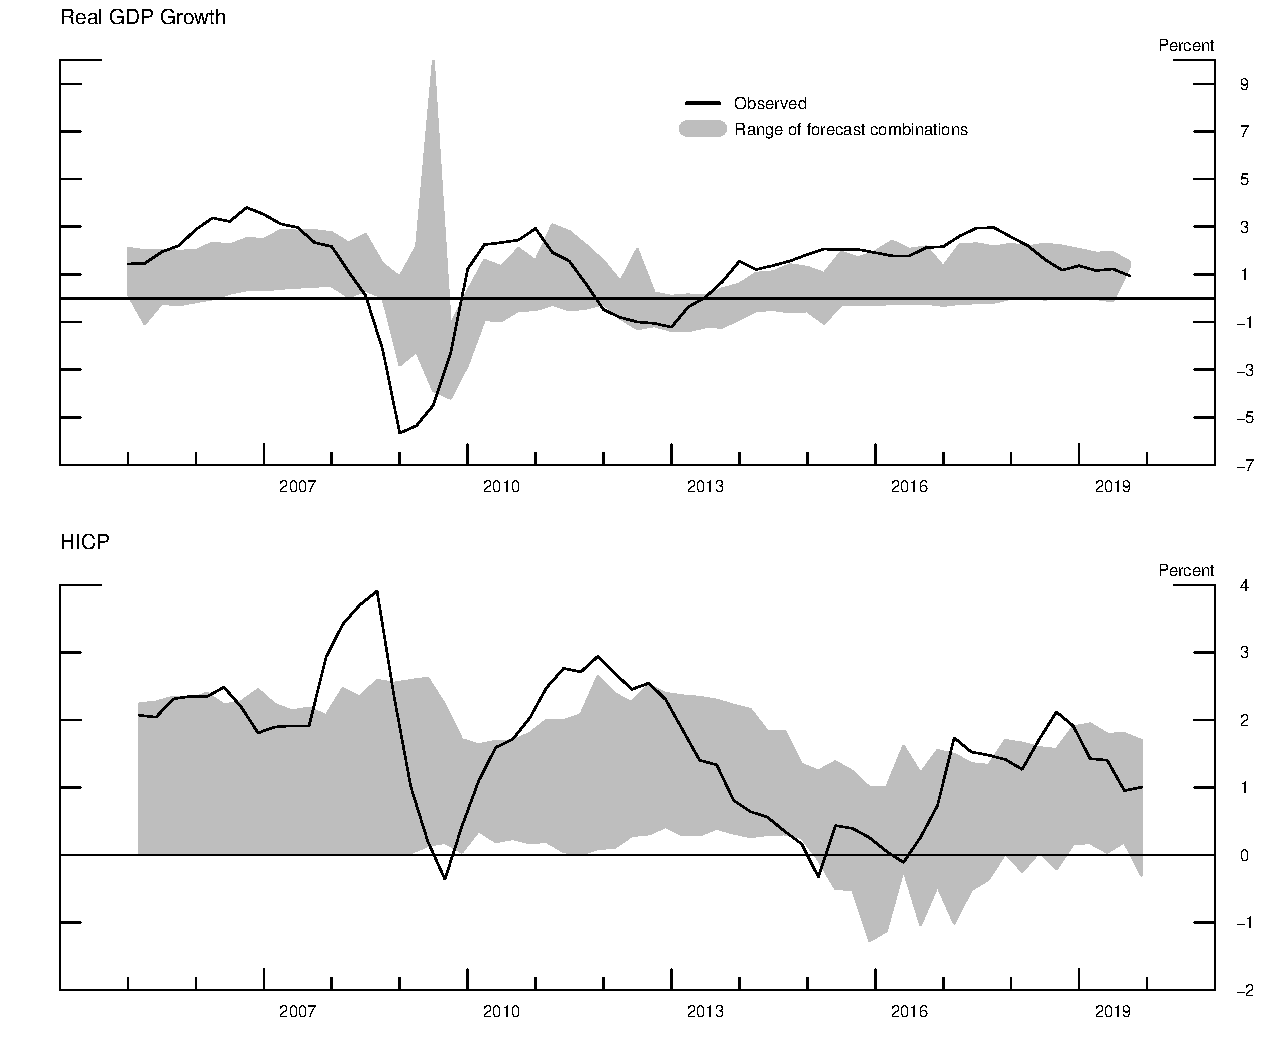
\includegraphics[width = .95\textwidth]{euroForecastChart_shaded.pdf}
\caption*{Quarterly, one-year-ahead, forecast combinations are shown from 2005 through 2019. The thick black line denotes the observed series and the grey shaded region identifies the range of forecast combination point estimates.}
\end{figure}

Figure \ref{fig:EuroForecasts} shows the one-year ahead forecast combinations for both changes in United States payroll employment and industrial production. 
% Table: Forecast Combination Results: European Survey of Professional Forecasters
\begin{table}[ht]
\caption{European Survey of Professional Forecasters combination results}
\label{tab:euroForecat}
\centerline{
\begin{tabular}{ccccc}
  \hline
  \hline
  Combination technique  & \multicolumn{2}{c}{HICP} & \multicolumn{2}{c}{Real GDP}\\
  \cmidrule(lr){2-3}\cmidrule(lr){4-5}
   & Relative MSE & Diebold-Mariano  & Relative MSE & Diebold-Mariano   \\
  \hline
    Mean Forecast & 1.00 & 1.00 & 1.00 & 1.00 \\
    Median Forecast & 1.00& 0.21  & 1.00  & 0.05$^\circ$  \\
    Lasso & 2.05 & 0.99 & 1.64  & 1.00\\ 
    peLasso & 2.27  & 1.00& 2.09  & 0.98  \\ 
    N1 & 0.81  & 0.04$^\circ$ & 0.88  & 0.15 \\ 
    N2 & 0.83 & 0.04$^\circ$ & 0.90 & 0.15 \\ 
    N3 & 0.82  & 0.03$^\circ$ & 0.91 & 0.14  \\  
    N4 & 0.83  & 0.02$^\circ$  & 0.91  & 0.13  \\ 
    Random Forest & 1.02  & 0.27  & 1.06  & 0.38  \\ 
    Boosted Tree & 0.97 & 0.13  & 0.96 & 0.21  \\
   \hline
   \hline
\end{tabular}}
\vspace{10pt}
\caption*{Notes: columns (2) and (4) report the RMSE of the combination method specified in column (1) divided by the RMSE the average survey forecast. A ratio less than one denotes the combination outperforming the uniform forecast. Columns (3) and (5) report the \cite{DM1995} p-value with the null hypothesis that the mean forecast is better than the model. $^\odot$, $^\circ$, $^\star$ denote DM statistics significant at the ten-percent, five-percent, and one-percent confidence level, respectively.}
\end{table}


Table \ref{tab:euroForecat} reports the relative root mean squared error (RMSE) and relative mean squared error (MSE) of forecast combination techniques, where relative denotes a ratio of forecast combination errors to uniform weight errors. By construction, a relative RMSE or MSE less than one signals a forecast combination technique superior to using uniform weights. We use both RMSE and MSE, as together they help us detect the presence of outliers in the errors. Table \ref{tab:euroForecat} also reports the \cite{DM1995} statistic p-value, testing the statistical significance of the difference in forecast combination errors. 

We find that the LASSO and peLASSO do not perform well, in terms of either RMSE or MSE. However, the LASSO-related N-best methods perform extremely well, with both RMSE and MSE being nearly eighty percent of those from uniform weights for forecasting HICP. Further, the N-best methods decrease forecast errors for the HICP at a statistically significant level, according to the Diebold-Mariano statistic. The N-best also achieve considerable success forecasting real GDP, reaching a relative MSE of 0.76. However, the forecast improvements generated by the N-best method for real GDP are not statistically significant according to the Deibold-Mariano statistic. We additionally find that the tree-methods do well, producing relative MSE's less than one, but they are not statistically significant. Although, it is notable that the boosted tree has a relative MSE of 0.78 for forecasting real GDP, second only to N1.   

\subsection{United States macroeconomic data}
In our second exercise, forecasting United States macroeconomic data, we find further evidence that nonlinear methods can outperform uniform weights and the median forecast combination. 

% Figure: (USA) One-step ahead forecasts
\begin{figure}[!htb]
\caption{United States macroeconomic series forecast combinations}\label{fig:USAForecast}
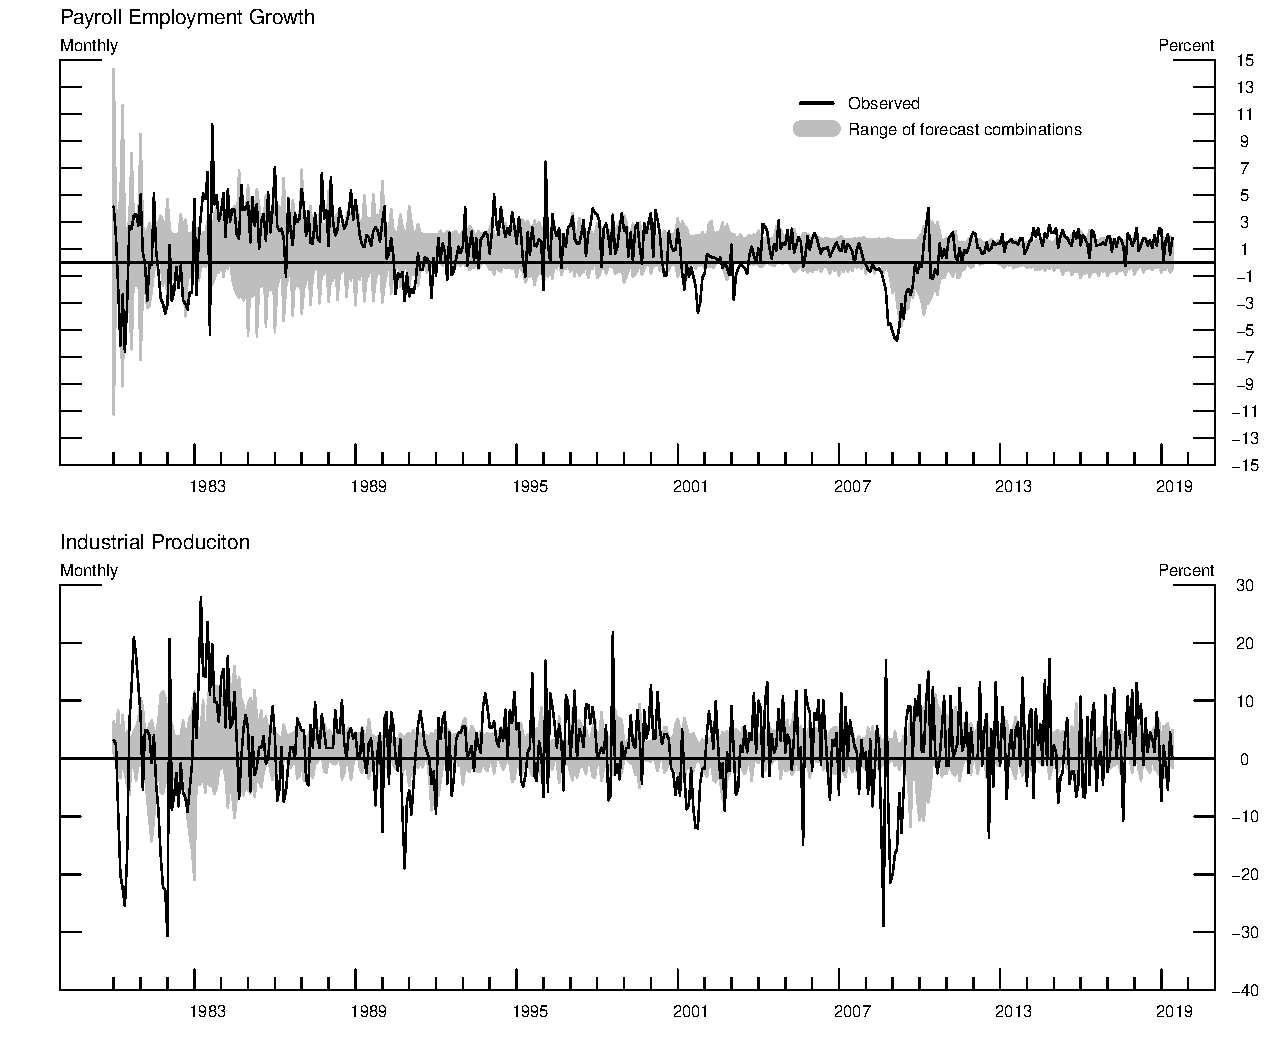
\includegraphics[width = .95\textwidth]{usaForecastChart_shaded.pdf}
\caption*{Monthly, one-year-ahead, forecast combinations are shown from 1980 through 2019. The thick black line denotes the observed series and the grey shaded region identifies the range of forecast combination point estimates.}
\end{figure}

Figure \ref{fig:USAForecast} shows the one-year ahead forecast combinations for both changes in United States payroll employment and industrial production. 

% Table: Forecast Combination Results: United States Macroeconomic Series - recursive model estimation
% latex table generated in R 3.6.1 by xtable 1.8-4 package
% Tue Jan 14 09:09:15 2020
\begin{table}[ht]
\caption{United States macroeconomic data forecast combination results}
\label{tab:usaForecastComparison}
\centerline{
\begin{tabular}{ccccccccc}
  \hline
  \hline
  Combination Technique  & \multicolumn{4}{c}{Employment} & \multicolumn{4}{c}{Industrial Production}\\
  \cmidrule(lr){2-5}\cmidrule(lr){6-9}
  & H = 1 & H = 6 & H = 12 & H = 24 & H = 1 & H = 6 & H = 12 & H = 24 \\
  %\hline
  %Time Series Models &&&&&\\
  %\hline
  %Historical Mean & 1.20 & 0.99 & 0.94 & 0.81 & 1.06 & 0.99 & 0.93 & 0.92 \\ 
  %Random Walk & 1.10 & 1.08 & 1.07 & 1.11 & 1.21 & 1.32 & 1.32 & 1.35 \\ 
  %Random Walk (w. drift) & 1.10 & 1.09 & 1.10 & 1.17 & 1.22 & 1.33 & 1.35 & 1.41 \\
  %Random Walk (w. season) & 1.26 & 1.10 & 1.07 & 1.11 & 1.38 & 1.34 & 1.32 & 1.35 \\ 
  %Exponential Smoothing & 0.92 & 0.93 & 0.99 & 1.00 & 1.02 & 1.15 & 1.18 & 1.19 \\ 
  %Theta Method & 5.06 & 5.06 & 5.20 & 5.98 & 1.51 & 1.32 & 1.20 & 1.20 \\ 
  %TBATS Method & 0.94 & 0.93 & 0.95 & 0.90 & 1.00 & 0.99 & 0.95 & 0.93 \\ 
  %STLM-AR & 0.98 & 0.93 & 0.93 & 0.85 & 1.09 & 1.02 & 0.95 & 0.94 \\ 
  %ARIMA & 0.95 & 0.93 & 0.95 & 0.86 & 1.01 & 0.99 & 0.94 & 0.92 \\ 
  %AR-Neural Network & 1.04 & 1.15 & 1.30 & 1.19 & 1.08 & 1.18 & 1.17 & 1.27 \\ 
  %\hline
  %Forecast Combinations &&&&&\\
  \hline
  %Mean Forecast & 1.00 & 1.00 & 1.00 & 1.00 & 1.00 & 1.00 & 1.00 & 1.00 \\ 
  Median Forecast & 0.91$^\star$ & 0.90$^\star$ & 0.90$^\star$ & 0.86$^\star$ & 1.00 & 0.99 & 0.96 & 0.96$^\star$ \\ 
  peLasso & 1.49 & 1.33 & 1.19 & 1.08 & 1.10 & 1.09 & 1.00 & 1.00 \\ 
  Lasso & 1.49 & 1.33 & 1.32 & 1.24 & 1.10 & 1.09 & 1.00 & 1.00 \\ 
  N1 & 0.94$^\odot$ & 0.99 & 0.94 & 0.82$^\star$ & 1.03 & 0.99 & 0.93$^\circ$ & 0.92$^\star$ \\ 
  N2 & 0.93$^\odot$ & 0.94$^\odot$ & 0.92$^\circ$ & 0.82$^\star$ & 1.02 & 0.99 & 0.93$^\star$ & 0.92$^\star$ \\ 
  N3 & 0.93$^\star$ & 0.92$^\star$ & 0.90$^\star$ & 0.82$^\star$ & 1.01 & 0.99 & 0.93$^\circ$ & 0.92$^\star$ \\ 
  N4 & 0.92$^\star$ & 0.90$^\star$ & 0.90$^\star$ & 0.82$^\star$ & 1.00 & 0.98 & 0.93$^\circ$ & 0.92$^\star$ \\ 
  %Neural Network & 1.09 & 0.92$^\odot$ & 0.90$^\circ$ & 0.78$^\star$ & 1.05 & 0.98 & 0.93$^\circ$ & 0.93$^\star$ \\
  Random Forest & 0.96 & 0.83$^\star$ & 0.80$^\star$ & 0.67$^\star$ & 0.99 & 0.96 & 0.91$^\circ$ & 0.93$^\circ$ \\ 
  Boosted Tree & 0.94$^\circ$ & 0.86$^\star$ & 0.83$^\circ$ & 0.72$^\star$ & 0.98$^\circ$ & 0.96 & 0.92$^\odot$ & 0.92$^\circ$ \\ 
  FFORMA & 1.19 & 0.73$^\odot$ & 0.64$^\circ$ & 0.48$^\star$ & 0.58$^\star$ & 0.37$^\star$ & 0.33$^\star$ & 0.37$^\star$ \\
  \hline
  \hline
\end{tabular}}
\caption*{Notes: forecast performance is reported as the ratio of the given forecast combination method's RMSE to the mean forecast's RMSE, such that a ratio less than one signals a forecast performance better than using uniform weights. $^\odot$, $^\circ$, $^\star$ denote \cite{DM1995} statistics significant at the ten-percent, five-percent, and one-percent confidence level, respectively, testing that the given forecast combination technique improves upon using uniform weights.}
\end{table}

Table \ref{tab:usaForecastComparison} reports the relative RMSE of forecast combination techniques across all four horizons for both changes in payroll employment and industrial production. The time series characteristic driven FFORMA the clear standout star of this exercise. We find that it strictly dominates all other combination techniques across all but one series-horizon pair. In fact, FFORMA averages an error ratio of 0.58 across all eight exercises, achieving a minimum of 0.33 for one-year ahead industrial production forecasts. The key difference between FFORMA and the other combination methods is that FFORMA aims to provide the best combination weights across many time series, appropriatley regularizing the weights to prevent overfitting to one time series, reducing noise. Table \ref{tab:usaForecastComparison} details results providing strong evidence that reducing noise through regularizing over many time series allows one to strictly dominate uniform combination weights. 

We further find that for all but one monthly variable-horizon pair, both simple tree-based methods outperform both mean and median forecast combination techniques. Particularly of note is the fact that for both tree-methods, across both payroll employment and industrial production, there appears to be a positive correlation between relative performance and horizon length. The random forest and boosted tree achieve RMSE ratios of 0.67 and 0.72 respectively when forecasting payroll employment two years ahead, the two greatest error improvements of the exercise. Almost all tree-based errors are better than the baseline at the ten-percent confidence level, as measured by the Diebold-Mariano statistic. The N-best techniques again perform well and the LASSO and peLASSO do not.

It is also important to note that the mean is being driven in part by an outlier in the underlying forecasts (indicated by the significant improvement by using the median) and does very poorly. In contrast, the tree-based and N-best techniques were given the same forecasts and were able to successfully ignore the poorly performing outliers, acting as a sanity check, or an automatic pooling method, on forecast inputs. Additionally, it appears that the relative performance of the tree-techniques increases as the number of observations increases (comparing monthly to quarterly results). This phenomenon may be driving by relatively large number of parameters inside the tree-techniques, but to definite conclusion would require more experiments, which we will leave open for future work. 

%\section{Measuring forecast performance and results}
%We find that ML techniques can outperform uniform weights in both an economically and statistically significant way. Further, we find that ML techniques are able to act as a reasonable sanity check on poor forecast inputs when uniform weights cannot. Results are presented in three stages, first we analyze results using the full sample of observations, second we remove recessions to determine the marginal effects of heterogeneous regimes, third we increase the number of quarterly observations to determine the marginal effects of estimation on small sample sizes.

%\subsection{Full-sample results}
%We first forecast real GDP, payroll employment, industrial production, and the price deflator with our nine time series models and then combine these models with our four forecast combination techniques.

%Figure \ref{fig:OneYearForecast} shows the one-year ahead time series forecasts and forecast combinations while Figure \ref{fig:OneStepForecast} shows the one-step ahead time series forecasts and forecast combinations. Both figures show that a subset of time series forecasts perform unreasonably until 1980, most likely needing a sufficient amount of observed data to be effective, and as a result, we chose to restrict our forecast analysis from 1980 through the present.

%Table \ref{tab:fullSampleRMSEMonthly} and Table \ref{tab:fullSampleRMSEQuarterly} display the root mean squared forecast error (RMSE) ratio of monthly and quarterly data respectively. All forecast performances are presented as a RMSE ratio against a simple AR(12) or AR(4) model, such that values less than one indicate an RMSE less than that of the simple AR. We find that for all but one monthly variable-horizon pair, a tree based method outperforms both mean and median forecast combination techniques. We note that the mean does very poorly and this is driven by the performance of the TBATS method. In contrast, the ML techniques were given the same forecasts and were able to successfully ignore the poorly performing TBATS method, acting as a sanity check, or an automatic pooling method, on forecast inputs. Further, the both tree-based methods outperform the explicit pooling methods, peLASSO and the average best (N1, using the best, and N4 using the four best) combinations, in almost all variable-horizon pairs. However, Table \ref{tab:fullSampleRMSEQuarterly} shows that there are only two quarterly variable-horizon pairs for which a ML combination is better than the mean and median forecast combination.

%Table \ref{tab:forecastComparisonFullSample} displays a direct comparison between ML forecast combinations and the mean forecast combination technique. The relative MSE column is the ratio between the mean squared forecast error (MSE) of the ML forecast combination and the mean forecast combination, such that a score less than one denotes a better performing ML combination. The Diebold-Mariano (Null is Mean) column shows the p-value from a \cite{DM1995} test with the null hypothesis being that the mean forecast combination is better than the ML combination.  The Diebold-Mariano (Null is ML) shows the p-value from a forecast error test with the null hypothesis being that the ML forecast combination is better than the mean combination. Table \ref{tab:forecastComparisonFullSample} highlights that the ML combinations greatly outperform the mean forecast combination for monthly variables. That is, all relative MSE ratios for monthly variables are less than one, and 12 of 16 Diebold-Mariano (Null is Mean) are statistically significant at the ten-percent level. Further, there is a clear trend that the ML combinations improve as the horizon increases; the MSE of payroll employment ML forecast combinations are approximately half of mean forecast combinations. However, this trend is not present in quarterly variable forecasts. In fact, only three relative MSE are less than one for quarterly variables.

%\subsection{Exclude recessions}
%We next remove NBER dated recessions so that me may evaluate a homogeneous set of forecasts generated in a single regime.
%Table \ref{tab:exRecRMSE} highlights that we find ML forecast combinations continue to outperform both uniform weights and median forecast combinations, while the boosted tree forecast combinations now outperform the mean forecast combinations for real GDP as well. Further, Table
%\ref{tab:forecastComparisonExRecSample} shows that the enhanced ML performance holds when comparing the two combination techniques directly, but not enough so to produce statistically significant Diebold-Mariono p-values. However, Diebold-Mariono do not confirm that mean forecast combinations outperform ML techniques. The facts that ML techniques can improve forecast combinations up to 18 percent, such as the boosted tree for real GDP eight quarters ahead, but not be statistically significant and the robust performance of ML on monthly variables suggests that a possible constraint on these nonlinear techniques may be the number of observations.

%\subsection{Simulate quarterly data}
%To evaluate if a limited number of observations may act as a constraint on the performance of ML combination techniques we estimate our ML forecast combinations on simulated quarterly data\footnote{We also run the experiment on weekly data, oil prices and the 10-year Treasury yield. We find robust results that ML techniques outperform mean forecasts. However, since these are financial series, we cannot isolate the large number of observations as driving the ML success. Results are presented in Appendix \ref{weeklyData}.}\footnote{We also look at the performance of different subsamples and find that ML performance is positively correlated with the number of observations previously realized in the time series.}. We run the same experiment as before, except each time we train (estimate) our ML models we first triple the number of observations via time series bagging \`{a} la \cite{BergmeirBagging2016}.

%Table \ref{tab:forecastComparisonExRecBootstrapped} shows that when increasing the number of observations and excluding recessions we find similar results for real GDP but have modestly increased the performance of ML techniques for the price deflator. These results suggest that ML techniques may be limited by a set of idiosyncratic series characteristics, primarily the number of observations.

\section{Conclusions}
We conduct two exercises to evaluate the ability of nonlinear forecast combination techniques. First, using the European Survey of Professional Forecasters in two real-time forecast combination exercises, we document that nonlinear models currently in forecast combination literature can outperform uniformly-weighted forecast combinations. 
Second, document robust evidence across 8 different real-time forecast exercises of United States macroeconomic data that nonlinear techniques can consistently outperform both uniform weights and median forecasts combinations. The two tree-based forecast combination methods introduced in this paper strictly dominate the mean forecast combination, across all eight exercises. Further, these tree-based methods can serve as a useful sanity check on poorly performing forecasts in a way that the uniform weights cannot. Additionally, it appears that the relative ability of tree-based methods, in comparison to simpler nonlinear techniques, increases as the number forecast observations increases. We also show that when the underlying forecast generating processes are available, then the feature augmented model averaging technique can  dominate all other forecast combination techniques. We attribute the success of the FFORMA to its ability to regularize forecast combination weights over many time series in such a way to reduce the possibility of over-fitting on one series, minimizing noise.  
In total, we document evidence that, in opposition to conventional forecasting wisdom, demonstrates that modern nonlinear forecast combination techniques produce more accurate forecasts than conventional approaches based on equal-weighed forecasts, breaking the so-called ``forecast combination puzzle''.

%\section{Conclusions}
 %We  first use a collection of nine standard time series models to forecast a collection of four important monthly and quarterly macroeconomic variables across four different horizons from 1970 to 2019. We then combine these forecasts with two nonlinear tree-based machine learning methods, random forest and boosted trees.  We find robust evidence across 16 different real-time forecast exercises that nonlinear techniques can consistently outperform both uniform weights and median forecasts combinations. Further, nonlinear tree-based methods can serve as a useful sanity check on poorly performing forecasts in a way that the uniform weights cannot. We also find that in cases with few observations (for example quarterly time series) we can trace any poor performance of the ML techniques to the presence of two regimes (i.e. mixing expansions and recessions) or a lack of training observations, which we propose to mitigate with bagged time series.

%In opposition to conventional forecasting wisdom, we further document  that combinations of real time forecasts from simple models using nonlinear weights calculated with machine learning algorithms produce more accurate forecasts than conventional approaches based on equal-weighed forecasts, breaking the so-called ``forecast combination puzzle''.


\newpage
%%%%%%%%%%%%%%%%%%%%%%%%%%%%%%%%%%%%%%%%%%%%%%%%%%%
% Exhibits
%%%%%%%%%%%%%%%%%%%%%%%%%%%%%%%%%%%%%%%%%%%%%%%%%%%



\clearpage

%--------------------------------------------------------
 \nocite{SW2009}
 \nocite{aiolfi2006persistence}
 \nocite{donaldson1996forecast}
\bibliography{NonLinReferences.bib}
%--------------------------------------------------------
\clearpage

\appendix
%--------------------------------------------------------
% Tree alogorithms
%--------------------------------------------------------
\section{Tree-based algorithms}\label{sec:treeML}

\RestyleAlgo{boxruled}
\begin{algorithm}[H]
\SetAlgoLined
\label{alg:randomForest}
\caption{Random Forest}
\For{$b = 1$ to $B$}{
Draw a bootstrap sample $Z^*$ of size $N$ from the training data\;
Grow a decision tree $T_b$ to the bootstrapped data, by recursively repeating the following steps for each terminal node of the tree, until the minimum node size $n_{min}$ is reached\;
\While{$n > n_{min}$}{
Select $m$ variables at random from the $p$ variables.\;
Pick the best variable/split point among the $m$.\;
Split the node into two daughter nodes.\;
}
}
Output the ensemble of trees ${T_b}^B_i$\;
 \vspace{2pt}
 \hrule\\
 \vspace{2pt}
 \textit{Source}: \cite{ElementsOfStatisticalLearning}
\end{algorithm}\ \\

\RestyleAlgo{boxruled}
\begin{algorithm}[H]
\SetAlgoLined
\label{alg:gbm}
\caption{Tree-based stochastic gradient boosting machine (Boosted Tree)}
Choose loss function $\Psi(y,f)$, learning rate $\lambda$, and tree depth $L$\;
% Initialize predictions: $f_i^{(0)} = log(\frac{\hat{p}}{1-\hat{p}})$\;
Instantiate simple decision tree $f(x)^{(0)}$\;
\For{iteration m = 1 ... K}{
Compute the gradient $\tilde{y_i} = \mathlarger{-(\frac{\partial \Psi(y_i,f(x_i)^{m-1})}{\partial f(x_i)^{m-1}})}$ for all observations $i$\;
Sample from training data without replacement \;
Train a tree model $h_i^{(m)}$ of depth $L$ on the random subset using the gradient as the outcome \;
Update the model $f_i^{(m)} = f_i^{(m-1)} + \lambda h_i^{(m)}$ \;
}
Instantiate trained model $f^{(K)}$ \;
 \vspace{2pt}
 \hrule\\
 \vspace{2pt}
 \textit{Source}: \cite{ElementsOfStatisticalLearning}
\end{algorithm}\ \\

\RestyleAlgo{boxruled}
\begin{algorithm}[H]
\SetAlgoLined
\label{alg:fforma}
 \caption{Feature-based forecast model averaging (FFORMA)} %of \cite{MMAHT2018}
 Offline Phase: Train the learning model\\
 \textbf{Input}\\ 
 \hspace{10pt} $R$: a set of $N$ observed time series, $\{x_1, x_2,...,x_N\}$, the reference set\;
 \hspace{10pt} $F$: a set of functions for calculating the time series features\;
 \hspace{10pt} $M$: a set of forecasting methods in the pool\;
 \textbf{Output} \\
 \hspace{10pt} FFORMA meta-learner: A function from the extracted features to a set of M weights, one for each forecasting method \;
 \vspace{10pt}
 \textit{Prepare the meta-data}\\
    \For{n = 1 to N}{
    Split $x_n \in R$  into a training period and test period\;
    Calculate the set of features $f_n \in F$ over the training period\;
    Fit each forecasting method $m \in M$ over the training period and generate forecasts over the test period\;
    Calculate forecast losses $L_{nm}$ over the test period\;
    }
 \vspace{10pt}
 \textit{Train the meta-learner, w}\\
 Train a learning model based on the meta-data and errors, by minimizing:
 $\argmin_w \sum^{N}_{n=1}\sum^{M}_{m=1} w(f_n)mL_{nm}$ \;
 \vspace{10pt}
 Online Phase: Forecast a new time series\\
 \textbf{Input}\\ 
 \hspace{10pt} FFORMA meta-learner from offline phase\;
 \textbf{Output} \\
 \hspace{10pt} Forecast the new time series $x_{new}$\;
 \vspace{10pt}
 \textit{Estimate forecasts}\\
    \For{ each $x_{new}$}{
    Calculate features $f_{new}$ by applying F\;
    Use the meta-learner to produce $w(f_{new})$ an $M$-vector of weights\;
    Compute the individual forecasts of $M$\;
    Combine individual forecasts using $w$ to generate final forecasts \;
    }
 \vspace{2pt}
 \hrule\\
 \vspace{2pt}
 \textit{Source}: \cite{MMAHT2018}
\end{algorithm} 


%--------------------------------------------------------
% Individual time series forecasts
%--------------------------------------------------------
\section{Time Series Forecasting Techniques}\label{app:TimeSeriesModels}
When conducting forecast combinations for US macroeconomic series, we estimate our own pool of constituent forecasts. We approximately follow \citeauthor{MMAHT2018} and estimate eleven univariate time-series models; a constant\footnote{Our experiments are all on stationary time series for which a constant is a reasonable forecast.}, three random walks, two exponential smoothing models, four ARIMA models, and one artificial neural network. All models are linear, except for the single-layer feed-forward neural network. These methods are standard, simple, and flexible models that have been shown to be successful in a variety of forecasting exercises. The complete list is

\begin{itemize}
    \item Mean %(meanf)
    \item Random walk %(naive)
    \item Random walk with drift %(dnaive)
    \item Seasonal random walk %(snaive)
    \item Automated exponential smoothing %(ets)
    \item TBATS model %(tbats)
    \item Theta method %(thetaf)
    \item AR(12)
    \item Automated ARIMA %(auto.arima)
    \item STLM-AR method %(stlm using model function ar)
    \item Autoregressive neural network %(nnetar)
\end{itemize}
%The R functions are given in parenthesis.

% Table: Forecast combination results: United States Macroeconomic Series: Individual time series
% latex table generated in R 3.6.1 by xtable 1.8-4 package
% Tue Jan 14 09:09:15 2020
\begin{table}[ht]
\caption{Forecast Combination Results: United States Macroeconomic Series}\label{tab:timeSeries}
\centerline{
\begin{tabular}{ccccccccc}
  \hline
  \hline
  Time Series Model & \multicolumn{4}{c}{Employment} & \multicolumn{4}{c}{Industrial Production}\\
  \cmidrule(lr){2-5}\cmidrule(lr){6-9}
  & H = 1 & H = 6 & H = 12 & H = 24 & H = 1 & H = 6 & H = 12 & H = 24 \\
  \hline
  Historical Mean & 1.20 & 0.99 & 0.94 & 0.81 & 1.06 & 0.99 & 0.93 & 0.92 \\ 
  Random Walk & 1.10 & 1.08 & 1.07 & 1.11 & 1.21 & 1.32 & 1.32 & 1.35 \\ 
  Random Walk (w. drift) & 1.10 & 1.09 & 1.10 & 1.17 & 1.22 & 1.33 & 1.35 & 1.41 \\
  Random Walk (w. season) & 1.26 & 1.10 & 1.07 & 1.11 & 1.38 & 1.34 & 1.32 & 1.35 \\ 
  Exponential Smoothing & 0.92 & 0.93 & 0.99 & 1.00 & 1.02 & 1.15 & 1.18 & 1.19 \\ 
  Theta Method & 5.06 & 5.06 & 5.20 & 5.98 & 1.51 & 1.32 & 1.20 & 1.20 \\ 
  TBATS Method & 0.94 & 0.93 & 0.95 & 0.90 & 1.00 & 0.99 & 0.95 & 0.93 \\ 
  STLM-AR & 0.98 & 0.93 & 0.93 & 0.85 & 1.09 & 1.02 & 0.95 & 0.94 \\ 
  ARIMA & 0.95 & 0.93 & 0.95 & 0.86 & 1.01 & 0.99 & 0.94 & 0.92 \\ 
  AR(12) & 0.94 &  0.91 & 0.90 & 0.82 & 1.01 & 1.00 & 0.94 & 0.92\\
  AR-Neural Network & 1.04 & 1.15 & 1.30 & 1.19 & 1.08 & 1.18 & 1.17 & 1.27 \\ 
  \hline
  \hline
\end{tabular}}
\caption*{Notes: forecast performance is reported as the ratio of the given forecast's RMSE to the mean forecast's RMSE, such that a ratio less than one signals a forecast performance better than using an unweighted average of all forecasts.}
\end{table}

The mean is the sample mean. Random walk is the previously observed growth rate. Random walk with drift is trend growth plus the previously observed deviation from trend. Seasonal random walk is the growth rate observed 12 periods past. The AR(12) is a standard 12-lag autoregressive forecasting regression. The automated ARIMA is a standard ARIMA model with $p$, $d$, and $q$ chosen to minimize Akaike's information criterion. The STLM-AR  applies a an AR (lag order chosen by standard information criterion) to a deseasonalized time series.  The autoregressive neural network is the average of twenty single-layer feed-forward networks (see \cite{ElementsOfStatisticalLearning} for a textbook treatment of simple single-layer neural networks).
The exponential smoothing model fits seasonal and trend components to a standard autoregressive state-space model (see \cite{autoETS2002}). TBATS uses the aforementioned exponential smoothing model, after controlling for  seasonal effects (see \cite{tbats2008}). The Theta method is a hybrid exponential smoothing and ARIMA model, as it decomposes time series and then uses either method to forecast the newly separated elements of the time series. Each model is re-estimated every period, using all available information up to date. Following \citet{MMAHT2018}, our forecasting models are trained using the \textsc{forecast} package in R (\citet{forecastPackage}) with default settings.

Table \ref{tab:timeSeries} shows the individual results for each constituent time series forecast in our model pool. As in our other analysis, all ratios are compared relative to the mean forecast combination. The Theta method is a clear outlier in its inability to forecast the monthly employment series. While all AR-based models (AR(12), Automated ARIMA, TBATs, and STLM-AR) are able to achieve success across all series and horizons. Lastly, the historical mean is able to minimize the forecast errors the most, compared to a simple average of all forecasts, when forecasting two-years ahead for both series. This may indicate that more sophisticated methods lose power or simply introduce too much noise as horizons extend.   

\newpage
%--------------------------------------------------------
% FFORMA informationn set robustness
%--------------------------------------------------------
\section{FFORMA informationn set robustness}\label{app:FFORMAInfoSet}

% Table: Forecast Combination Results: United States Macroeconomic Series - one-time model estimation
% latex table generated in R 3.6.1 by xtable 1.8-4 package
% Tue Jan 14 09:09:15 2020
\begin{table}[ht]
\caption{United States macroeconomic data forecast combination results ---
one-time model estimation}
\label{tab:fformaRobustness_1}
\centerline{
\begin{tabular}{ccccccccc}
  \hline
  \hline
  Combination Technique  & \multicolumn{4}{c}{Employment} & \multicolumn{4}{c}{Industrial Production}\\
  \cmidrule(lr){2-5}\cmidrule(lr){6-9}
  & H = 1 & H = 6 & H = 12 & H = 24 & H = 1 & H = 6 & H = 12 & H = 24 \\
  \hline
  %Median Forecast & 0.86$^\star$ & 0.83$^\star$ & 0.89$^\star$ & 0.89$^\circ$ & 0.99 & 0.97 & 0.92$^\circ$ & 0.9$^\star$\\ 
  peLasso & 2.13  & 1.89 & 1.46 & 1.2 & 1.19 &  1.29 & 0.96 & 1.03 \\ 
  Lasso & 2.2 & 1.9 & 2.15 & 2.28 & 1.18 & 1.29 & 0.97 & 0.97 \\ 
  Random Forest & 1.12 & 0.93 & 1.45 & 1.19 & 1.11 & 1.22 & 1.05 & 1.04  \\ 
  Boosted Tree & 1.78 & 1.07 & 1.61 & 1.36 & 1.07 & 1.16 & 1.16 & 1.19  \\ 
  FFORMA & 1.24 & 0.82 & 0.79 & 0.67$^\circ$ & 0.49$^\star$ & 0.28$^\star$ & 0.29$^\star$ & 0.30$^\star$ \\
  \hline
  \hline
\end{tabular}}
\caption*{Notes: forecast performance is reported as the ratio of the given forecast combination method's RMSE to the mean forecast's RMSE, such that a ratio less than one signals a forecast performance better than using uniform weights. $^\odot$, $^\circ$, $^\star$ denote \cite{DM1995} statistics significant at the ten-percent, five-percent, and one-percent confidence level, respectively, testing that the given forecast combination technique improves upon using uniform weights. Machines are trained on forecast errors from 1970 through 1979, and forecast combinations from 1980 through 2019 are evaluated.}
\end{table}

% Table: Forecast Combination Results: United States Macroeconomic Series - one-time model estimation
% latex table generated in R 3.6.1 by xtable 1.8-4 package
% Tue Jan 14 09:09:15 2020
\begin{table}[ht]
\caption{United States macroeconomic data forecast combination results ---
one-time model estimation}
\label{tab:fformaRobustness_2}
\centerline{
\begin{tabular}{ccccccccc}
  \hline
  \hline
  Combination Technique  & \multicolumn{4}{c}{Employment} & \multicolumn{4}{c}{Industrial Production}\\
  \cmidrule(lr){2-5}\cmidrule(lr){6-9}
  & H = 1 & H = 6 & H = 12 & H = 24 & H = 1 & H = 6 & H = 12 & H = 24 \\
  \hline
  %Median Forecast & 0.86$^\star$ & 0.83$^\star$ & 0.89$^\star$ & 0.89$^\circ$ & 0.99 & 0.97 & 0.92$^\circ$ & 0.9$^\star$\\ 
  peLasso & 3.05 & 2.03 & 1.45 & 0.93 & 1.15 & 1.24 & 1 & 0.98 \\ 
  Lasso & 2.99 & 2.01 & 1.49 & 1.07 & 1.16 & 1.24 & 1.02 & 0.99 \\ 
  Random Forest & 2.03 & 2.21 & 2.77 & 2.52 & 1.08 & 1 & 1.31 & 0.90$^\odot$  \\ 
  Boosted Tree & 5.68 & 3.89 & 2.59 & 2.15 & 0.98 & 0.99 & 1.13& 0.91 \\ 
  FFORMA & 1.92 & 1 & 0.73 & 0.59 & 0.36$^\star$ & 0.30$^\star$ & 0.29$^\star$ & 0.26$^\star$ \\
  \hline
  \hline
\end{tabular}}
\caption*{Notes: forecast performance is reported as the ratio of the given forecast combination method's RMSE to the mean forecast's RMSE, such that a ratio less than one signals a forecast performance better than using uniform weights. $^\odot$, $^\circ$, $^\star$ denote \cite{DM1995} statistics significant at the ten-percent, five-percent, and one-percent confidence level, respectively, testing that the given forecast combination technique improves upon using uniform weights. Machines are trained on forecast errors from 1970 through 1979, and forecast combinations from 1980 through 2019 are evaluated.}
\end{table}

We train the FFORMA machine with 1,000 randomly selected series from the M4 competition, which ran in 2018. As a result, it is possible that the FFORMA is drawing its success from simply having seen enough macroeconomic series through 2018 that it can redraw industrial production and employment across our testing period. That is, the FFORMA machine may be contaminated with a future-biased information set. To evaluate the results of the FFORMA, expunging any possible future-bias, we replicate our primary experiment, but with nonlinear techniques estimated on data only running from 1) 1970 through 1979, and 2) 1970 through 2000. However, noting that this will severely restrict the number of observations available to FFORMA, we allow the machine to train over the approximately 12,000 or 9,000 series out of the 100,000 M4 competition series, with data available from 1970 through 1979 or 1970 through 2000, respectively. 

Table \ref{tab:fformaRobustness_1} shows the results from our FFORMA robustness check when using training data form 1970 through 1980. Even when controlling for any possible future bias in the function estimation, FFORMA is by the best performing forecast combination method. In fact, restricting the length of the training time series apears to have had no qualitative affect on the performance of the algorithm. Table \ref{tab:usaForecastComparison} and Table \ref{tab:fformaRobustness_1} report very similar FFORMA results.  

Table \ref{tab:fformaRobustness_2} shows the results from our FFORMA robustness check when using training data form 1970 through 2000. Similar to the smaller sample set, FFORMA is by the best performing forecast combination method. Again, restricting the length of the training time series appears to have had no qualitative affect on the performance of the algorithm. Table \ref{tab:usaForecastComparison} and Table \ref{tab:fformaRobustness} report very similar FFORMA results. 

%%%%%%%%%%%%%%%%%%%%%%%%%%%%%%%%%%%%%%%%%%%%%%%%%%%
\end{document} 